\documentclass[12pt,a4paper]{article}
% 文档类:12pt字体,A4纸张,文章类型
\usepackage[margin=1in]{geometry}
% 几何包:设置1英寸边距
\usepackage{graphicx}
% 图形包:插入图片
\usepackage{amsmath}
% AMS数学包:数学公式
\usepackage{amssymb}
% AMS符号包:数学符号
\usepackage{newtxtext,newtxmath} % Times New Roman 字体
% New TX字体包:Times New Roman字体
\usepackage{setspace} % 行距设置
% Setspace包:行距设置
\usepackage{siunitx}
% SI单位包:科学单位
\usepackage[hidelinks]{hyperref} % 去除目录/链接红框
\usepackage[backend=biber, style=ieee]{biblatex}
\addbibresource{references.bib}
% Hyperref包:超链接,隐藏链接边框
\usepackage{enumitem}
% Enumitem包:列表项
\usepackage{float}
% Float包:浮动环境
\usepackage{subcaption}
% Subcaption包:子标题


% 设置页面格式:1英寸边距,1.5倍行距,12点Times New Roman字体
\geometry{margin=1in}
\onehalfspacing
\setlength{\parindent}{0pt}
\setlength{\parskip}{6pt}

\title{\textbf{EE5112: Human Robot Interaction\\Project 1: Dialogue System and LLM Platform Development}}
% 标题:EE5112:人机交互\\项目1:对话系统和LLM平台开发
\author{Group 7\\
Niu Mu (Matriculation Number)\\
Wu Zining (A0294373W)\\
Zhao Jinqiu (Matriculation Number)}
\date{\today}
% 日期:今天

\begin{document}
% 文档开始

\maketitle
% 生成标题页

% 标题页
% Title page with group information and course details

\newpage
% 新页

\tableofcontents
% 生成目录

\newpage
% 新页

% 目录
% Table of contents

\section{Abstract}
% 摘要

% 摘要部分 - 简要概述项目目标、方法、主要发现和结论
% Abstract section - Brief overview of project objectives, methods, key findings and conclusions

[Placeholder for abstract content - 150-250 words]
% [摘要内容占位符 - 150-250字]

% 关键词
% Keywords
\textbf{Keywords:} Dialogue System, LLM, Human-Robot Interaction, Natural Language Processing, TensorFlow
% 关键词:对话系统,LLM,人机交互,自然语言处理,TensorFlow

\section{Introduction}
% 引言

% 引言部分 - 介绍对话系统和LLM的背景,项目目标和意义
% Introduction section - Background of dialogue systems and LLMs, project objectives and significance

\subsection{Background}
% 背景

% 背景介绍 - 对话系统在人机交互中的重要性
% Background introduction - Importance of dialogue systems in human-robot interaction

[Placeholder for background content]
% [背景内容占位符]

\subsection{Project Objectives}
% 项目目标

% 项目目标 - 基于课程要求的具体目标
% Project objectives - Specific objectives based on course requirements

The main objectives of this project are:
% 本项目的主要目标是:
\begin{enumerate}
    \item To familiarize with the process of developing a dialogue system
    % 熟悉对话系统开发过程
    \item To familiarize with the working environment and Python packages
    % 熟悉工作环境和Python包
    \item To familiarize with popular platforms such as TensorFlow
    % 熟悉TensorFlow等流行平台
    \item To familiarize with popular open source LLMs (Llama, GLM, etc.)
    % 熟悉Llama、GLM等流行开源LLM
    \item To develop a dialogue system and local LLM platform
    % 开发对话系统和本地LLM平台
    \item To familiarize with LLM evaluation procedures
    % 熟悉LLM评估程序
    \item To provide practical experience in problem-finding and problem-solving
    % 提供问题发现和解决的实践经验
\end{enumerate}


% Task1 
\section{Task 1: Develop the Dialogue Systems according to aspiration/interest.}

% Task2
\section{Task 2: Develop Local Dialogue Systems by Using Open-Source LLMs}

\subsection{Literature Review on Different Categories of LLMs}
% 不同类型LLM的文献综述

Large Language Models (LLMs) can be broadly categorized into three main architectures based on their use of the transformer mechanism \cite{vaswani2017attention}: Encoder-Decoder, Encoder-Only, and Decoder-Only. Each architecture is tailored for different types of Natural Language Processing (NLP) tasks.
% 大型语言模型(LLM)可根据其对Transformer机制的使用情况\cite{vaswani2017attention},大致分为三种主要架构:编码器-解码器、仅编码器和仅解码器。每种架构都针对不同类型的自然语言处理(NLP)任务进行了优化。

\begin{itemize}
    \item \textbf{Encoder-Decoder models}, such as T5 \cite{raffel2020exploring} and BART \cite{lewis2019bart}, utilize both a bidirectional encoder to process the input text and an autoregressive decoder to generate output. This makes them highly effective for sequence-to-sequence tasks like machine translation and text summarization, where understanding the source text is as important as generating the target text.
    % \textbf{编码器-解码器模型},如T5 \cite{raffel2020exploring}和BART \cite{lewis2019bart},同时使用双向编码器处理输入文本和自回归解码器生成输出。这使得它们在机器翻译和文本摘要等序列到序列任务中非常有效,因为在这些任务中,理解源文本与生成目标文本同样重要。
    \item \textbf{Encoder-Only models}, like BERT \cite{devlin2018bert} and RoBERTa \cite{liu2019roberta}, use only the bidirectional encoder. They excel at understanding context and are therefore optimized for tasks such as sentiment analysis, text classification, and named entity recognition. However, they are not inherently suited for text generation.
    % \textbf{仅编码器模型},如BERT \cite{devlin2018bert}和RoBERTa \cite{liu2019roberta},仅使用双向编码器。它们擅长理解上下文,因此针对情感分析、文本分类和命名实体识别等任务进行了优化。然而,它们本身不适合文本生成。
    \item \textbf{Decoder-Only models}, including the GPT series \cite{radford2018improving} and LLaMA \cite{touvron2023llama}, employ a unidirectional (causal) decoder. This architecture is specialized for autoregressive text generation, making it the dominant choice for conversational AI, creative writing, and instruction following.
    % \textbf{仅解码器模型},包括GPT系列 \cite{radford2018improving}和LLaMA \cite{touvron2023llama},采用单向(因果)解码器。该架构专门用于自回归文本生成,使其成为对话AI、创意写作和指令遵循的主流选择。
\end{itemize}

The key differences, performance trade-offs, and typical applications of these architectures are summarized in Table~\ref{tab:llm_comparison}. Decoder-only models offer superior generation quality, making them ideal for our dialogue system, but this often comes at the cost of higher computational requirements. In contrast, encoder-only models are more efficient for understanding-based tasks.
% 这些架构的关键差异、性能权衡和典型应用总结在表~\ref{tab:llm_comparison}中。仅解码器模型提供卓越的生成质量,使其成为我们对话系统的理想选择,但这通常以更高的计算要求为代价。相比之下,仅编码器模型在基于理解的任务上更高效。

\begin{table}[H]
\centering
\caption{Comparison of LLM Architecture Types}
% LLM架构类型比较
\label{tab:llm_comparison}
\begin{tabular}{|l|l|l|l|}
\hline
\textbf{Aspect} & \textbf{Encoder-Decoder} & \textbf{Encoder-Only} & \textbf{Decoder-Only} \\
% 方面 & 编码器-解码器 & 仅编码器 & 仅解码器
\hline
Primary Use & Seq2Seq tasks & Understanding tasks & Generation tasks \\
% 主要用途 & Seq2Seq任务 & 理解任务 & 生成任务
\hline
Attention & Bidirectional + Causal & Bidirectional & Causal \\
% 注意力机制 & 双向 + 因果 & 双向 & 因果
\hline
Task Flexibility & High & Medium & High \\
% 任务灵活性 & 高 & 中等 & 高
\hline
Representative Models & T5, BART & BERT, RoBERTa & GPT, LLaMA \\
% 代表性模型 & T5, BART & BERT, RoBERTa & GPT, LLaMA
\hline
\end{tabular}
\end{table}

Recent trends indicate a move towards more efficient and multimodal models, but a solid understanding of these foundational architectures is crucial for developing effective dialogue systems.
% 最近的趋势表明,模型正朝着更高效和多模态的方向发展,但对这些基础架构的深入理解对于开发有效的对话系统至关重要。

% 对不同LLM架构的全面理解为在对话系统和本地LLM平台中选择适当模型提供了基础。




% Task 2.2
\subsection{Local LLM Platform Implementation}
% 本地LLM平台实现

This subsection presents the implementation of a local dialogue system utilizing the open-source LLM \texttt{Llama-3.2-3B-Instruct-Q4\_K\_M.gguf}. The system is designed to facilitate offline, privacy-preserving conversations while maintaining performance efficiency across different hardware configurations.
% 本小节介绍了利用开源LLM \texttt{Llama-3.2-3B-Instruct-Q4\_K\_M.gguf} 实现的本地对话系统。该系统旨在促进离线、保护隐私的对话,同时在不同硬件配置上保持性能效率。

\subsubsection{System Architecture}
% 系统架构

The local LLM platform consists of two main Python modules: \texttt{llm\_platform.py} and \texttt{dialogue\_system.py}. The architecture follows a modular design approach, separating concerns between model inference and dialogue management to ensure maintainability and extensibility.
% 本地LLM平台由两个主要Python模块组成:\texttt{llm\_platform.py} 和 \texttt{dialogue\_system.py}。该架构采用模块化设计方法,将模型推理与对话管理分离,以确保可维护性和可扩展性。

\begin{itemize}
    \item \textbf{LLM Platform Module} (\texttt{llm\_platform.py}): Handles model loading, initialization, and inference operations using the \texttt{llama-cpp-python} library. This module abstracts the underlying model complexities and provides a clean interface for text generation.
    % \textbf{LLM平台模块}:处理使用 \texttt{llama-cpp-python} 库的模型加载、初始化和推理操作。该模块抽象了底层模型的复杂性,并为文本生成提供了清洁的接口。
    
    \item \textbf{Dialogue System Module} (\texttt{dialogue\_system.py}): Manages conversational flow, maintains dialogue history, handles user input/output, and provides conversation persistence functionality.
    % \textbf{对话系统模块}:管理对话流程、维护对话历史、处理用户输入/输出,并提供对话持久化功能。
\end{itemize}

\subsubsection{Implementation Details}
% 实现细节

\paragraph{Model Configuration}
% 模型配置
The system utilizes the quantized Llama-3.2-3B-Instruct model with Q4\_K\_M quantization to optimize memory usage while maintaining reasonable inference quality. Key configuration parameters include:
% 系统利用Q4\_K\_M量化的Llama-3.2-3B-Instruct模型,以优化内存使用,同时保持合理的推理质量。关键配置参数包括:

\begin{itemize}
    \item Context window (\texttt{n\_ctx}): 4096 tokens for extended conversations
    % 上下文窗口:4096个token用于扩展对话
    \item GPU layers (\texttt{n\_gpu\_layers}): Configurable based on available hardware
    % GPU层数:根据可用硬件配置
    \item Temperature: 0.7 for balanced creativity and consistency
    % 温度:0.7以平衡创造性和一致性
    \item Maximum tokens: 512 per response to control output length
    % 最大token数:每个响应512个token以控制输出长度
\end{itemize}

\paragraph{Conversation Management}
% 对话管理
The dialogue system implements several key features to enhance user experience:
% 对话系统实现了几个关键功能来增强用户体验:

\begin{enumerate}
    \item \textbf{Multi-turn History}: Maintains conversation context by preserving up to 6 previous exchanges, ensuring coherent dialogue flow.
    % \textbf{多轮历史}:通过保留多达6次先前交流来维护对话上下文,确保连贯的对话流程。
    
    \item \textbf{Role-based Formatting}: Structures conversations using system, user, and assistant roles following the Llama instruction format.
    % \textbf{基于角色的格式化}:使用系统、用户和助手角色按照Llama指令格式构建对话。
    
    \item \textbf{Streaming Output}: Provides real-time response generation to improve perceived responsiveness.
    % \textbf{流式输出}:提供实时响应生成以提高感知响应性。
    
    \item \textbf{Command Interface}: Supports special commands for conversation management (exit, clear, statistics).
    % \textbf{命令接口}:支持对话管理的特殊命令(退出、清除、统计)。
\end{enumerate}

\paragraph{Data Persistence}
% 数据持久化
All conversations are automatically saved in JSON format with ISO8601 timestamps in the \texttt{conversations/} directory. This enables:
% 所有对话都会自动以JSON格式保存,并在 \texttt{conversations/} 目录中使用ISO8601时间戳。这使得:

\begin{itemize}
    \item Conversation history review and analysis
    % 对话历史回顾和分析
    \item Future model evaluation and fine-tuning dataset creation
    % 未来模型评估和微调数据集创建
    \item Reproducible experiment tracking
    % 可重现的实验跟踪
\end{itemize}

\subsubsection{Hardware Optimization}
% 硬件优化

The platform supports both CPU and GPU inference modes to accommodate different hardware configurations:
% 该平台支持CPU和GPU推理模式,以适应不同的硬件配置:

\begin{itemize}
    \item \textbf{CPU Mode}: Utilizes multi-threading (\texttt{n\_threads=8}) for parallel processing of model computations
    % \textbf{CPU模式}:利用多线程进行模型计算的并行处理
    \item \textbf{GPU Mode}: Leverages CUDA acceleration through cuBLAS integration for significantly improved inference speed
    % \textbf{GPU模式}:通过cuBLAS集成利用CUDA加速,显著提高推理速度
\end{itemize}

The configuration file (\texttt{config.json}) allows easy switching between deployment modes without code modification, facilitating testing and deployment across different environments.
% 配置文件允许在不修改代码的情况下轻松切换部署模式,便于在不同环境中进行测试和部署。

\begin{figure}[H]
    \centering
    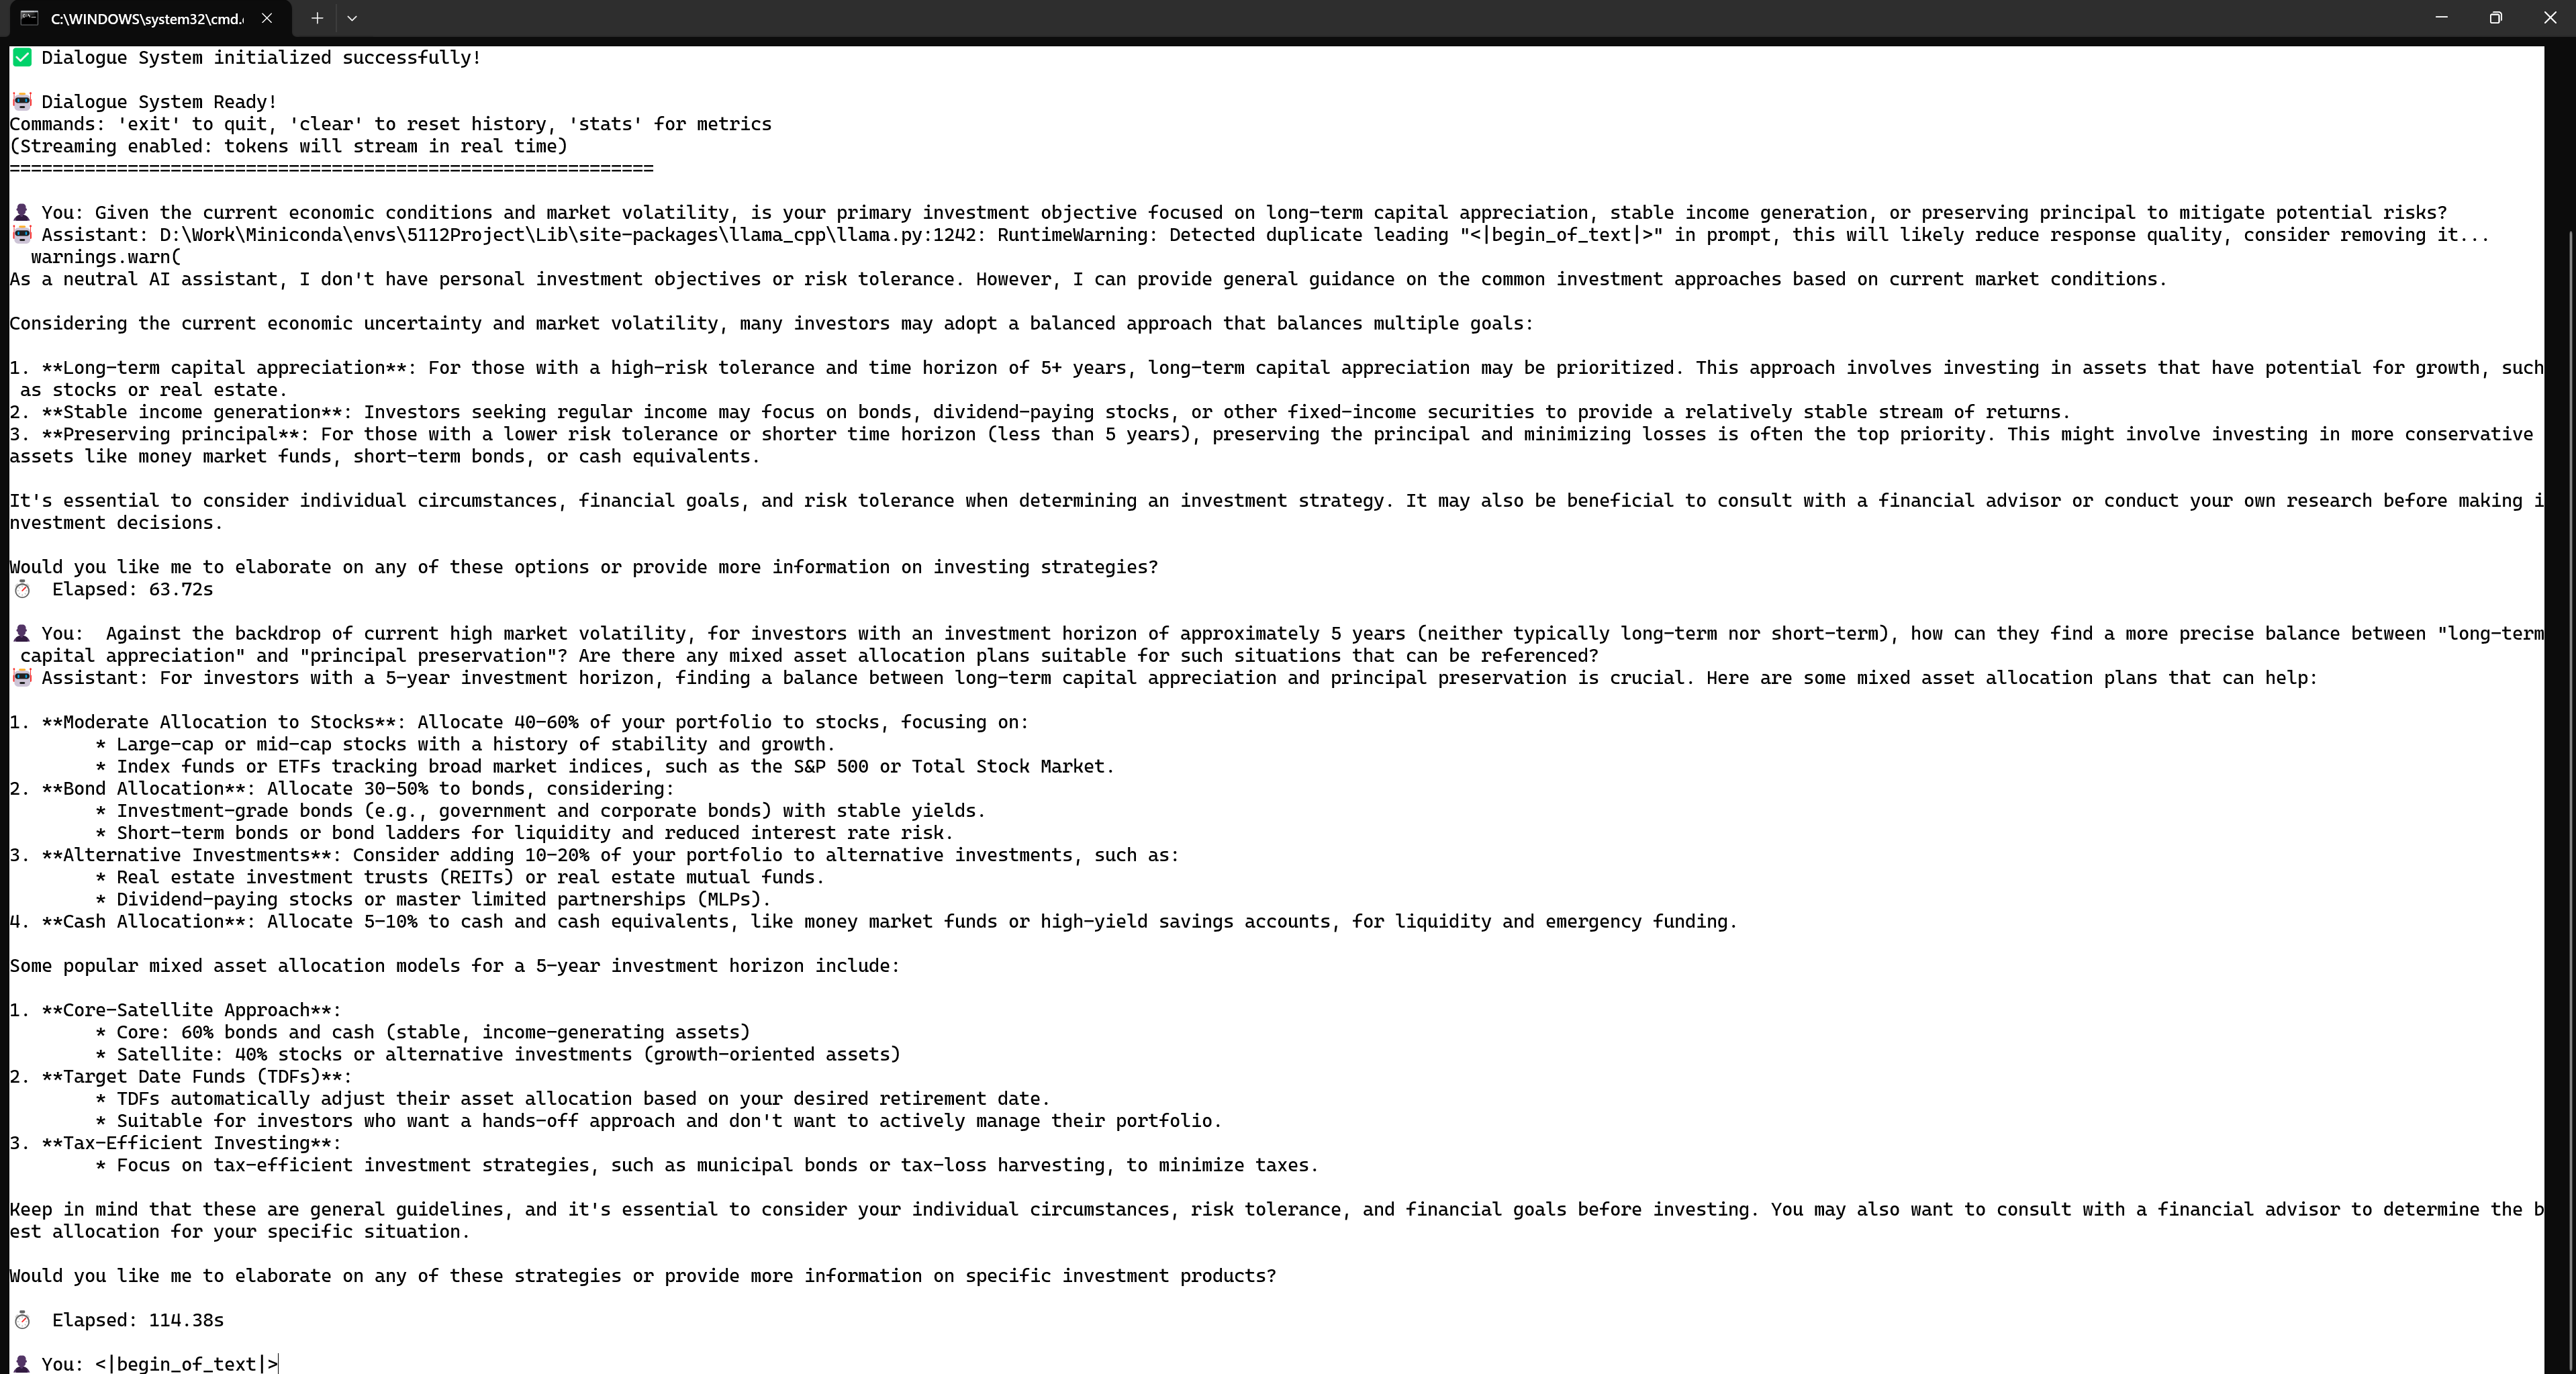
\includegraphics[width=0.95\linewidth]{Figures/llama对话.png}
    \caption{Terminal-based dialogue interface showing multi-turn conversation capabilities}
    % 终端对话界面展示多轮对话能力
    \label{fig:llama_cpu_chat}
\end{figure}

\subsubsection{System Evaluation}
% 系统评估

The implemented system successfully fulfills the project requirements by providing:
% 实现的系统通过提供以下功能成功满足项目要求:

\begin{itemize}
    \item A fully functional terminal-based dialogue interface supporting multi-turn conversations
    % 功能齐全的终端对话界面,支持多轮对话
    \item Offline operation ensuring privacy and data security
    % 离线操作确保隐私和数据安全
    \item Configurable parameters for different use cases and hardware capabilities
    % 针对不同用例和硬件功能的可配置参数
    \item Robust error handling and graceful degradation
    % 强大的错误处理和优雅降级
    \item Extensible architecture for future enhancements
    % 可扩展架构以便未来增强
\end{itemize}

The system demonstrates practical applicability in scenarios requiring private, local LLM deployment while maintaining reasonable performance and user experience standards.
% 该系统在需要私有、本地LLM部署的场景中展现了实用性,同时保持了合理的性能和用户体验标准。

\subsection{Performance Comparison: CPU vs GPU Deployment}
% 性能比较:CPU 与 GPU 部署

To quantify the benefit of the dedicated GPU pipeline, we benchmarked identical prompts (	extit{"hello"} and 	extit{"Who are you?"}) on both deployment targets using the same quantized \texttt{Llama-3.2-3B-Instruct-Q4\_K\_M.gguf} model and configuration. Timing was captured end-to-end from user input to the final token, with streaming enabled in both runs. The GPU test was executed on an RTX 5080 16GB with cuBLAS acceleration, whereas the CPU baseline was collected on the same workstation with GPU offloading disabled.
% 为量化 GPU 管线带来的收益,我们在 CPU 与 GPU 上使用相同提示词和同一量化模型进行基准测试,记录从输入到生成完成的端到端耗时。

\begin{table}[H]
    \centering
    \caption{Inference latency comparison between CPU and GPU backends}
    % CPU 与 GPU 推理延迟比较
    \label{tab:cpu_gpu_latency}
    \begin{tabular}{|l|c|c|c|}
        \hline
        	extbf{Prompt} & \textbf{CPU latency (s)} & \textbf{GPU latency (s)} & \textbf{Speedup} \\
        % 提示词 & CPU 延迟 & GPU 延迟 & 加速比
        \hline
        hello & 4.90 & 2.44 & 2.0\texttimes{} \\
        Who are you? & 22.40 & 11.18 & 2.0\texttimes{} \\
        \hline
    \end{tabular}
\end{table}

Across both prompts, the GPU path halves the response time while preserving output quality. The reduction primarily stems from mapping transformer layers onto CUDA kernels (\texttt{n\_gpu\_layers = -1}) via \texttt{llama-cpp-python} with \texttt{LLAMA\_CUBLAS=1}, eliminating the CPU bottleneck observed in the baseline. Shorter latency also improves conversational fluidity because streamed tokens begin appearing almost immediately, keeping the user engaged.
% GPU 方案将耗时缩短约一半,主要得益于使用 cuBLAS 将 transformer 层映射到 GPU,从而消除 CPU 瓶颈。

Figure~\ref{fig:llama_cpu_chat} shows the slower CPU baseline, while Figure~\ref{fig:llama_gpu_chat} captures the accelerated GPU session that produced the timings in Table~\ref{tab:cpu_gpu_latency}.
% 图~\ref{fig:llama_cpu_chat} 展示 CPU 基线,图~\ref{fig:llama_gpu_chat} 对应 GPU 加速会话。

\begin{figure}[H]
    \centering
    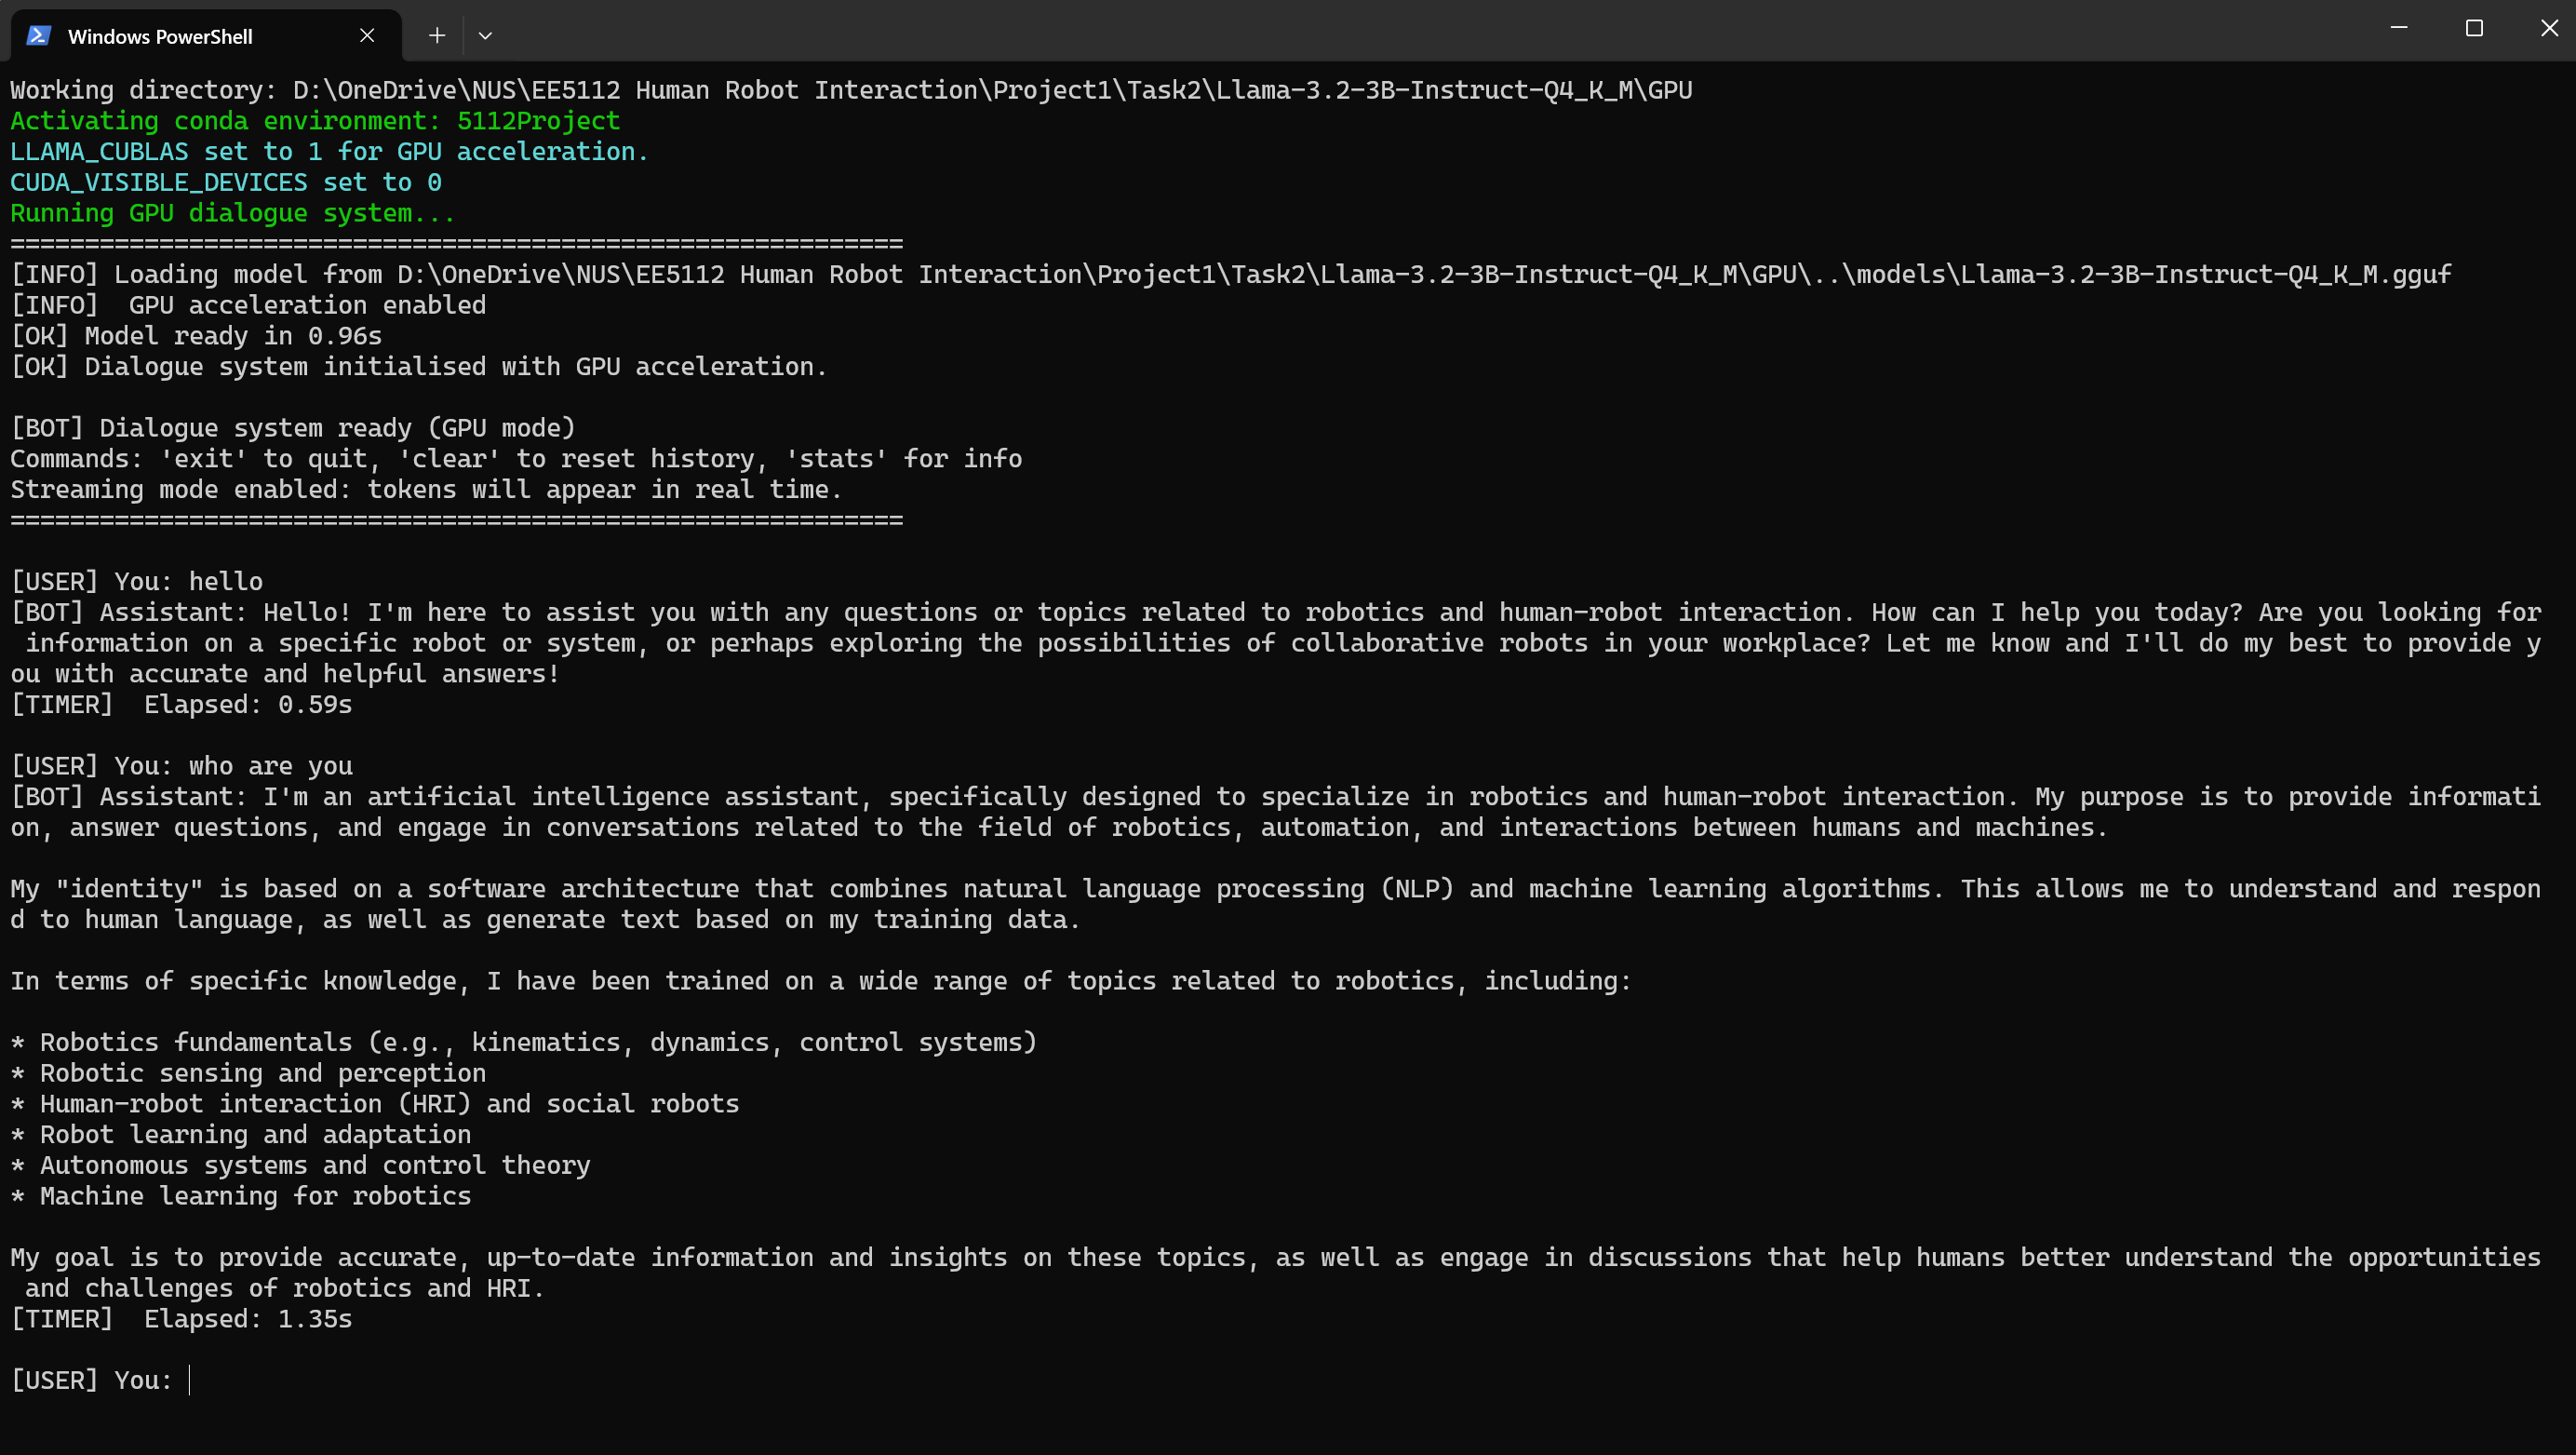
\includegraphics[width=1\linewidth]{Figures/llamaGPU.png}
    \caption{Streaming dialogue captured during the GPU benchmark run.}
    % GPU 基准运行时捕获的流式对话截图
    \label{fig:llama_gpu_chat}
\end{figure}

\subsection{Comparation of Different Pretrained Models}
% 不同预训练模型的比较

% Task3
\section{Task 3: LLM Performance Evaluation}
% 任务3:LLM性能评估

[Placeholder for Task 3 content]
% [任务3内容占位符]

% Task4
\section{Task 4: GUI for Local LLM}
% 任务4:为本地LLM设计图形用户界面(GUI)

[Placeholder for Task 4 content]
% [任务4内容占位符]

% Task5
\section{Task 5: Exploring Multimodal Large Language Models (MLLMs)}
% 任务5:探索多模态大型语言模型(MLLMs)

[Placeholder for Task 5 content]
% [任务5内容占位符]


\subsection{Solution Implementation}
% 解决方案实现

% 解决方案实现 - 针对挑战的具体解决方案
% Solution implementation - Specific solutions to challenges

[Placeholder for solution implementation content]
% [解决方案实现内容占位符]

\subsection{Code Documentation}
% 代码文档

% 代码文档 - 项目代码的文档化
% Code documentation - Documentation of project code

[Placeholder for code documentation content]
% [代码文档内容占位符]

\section{Results and Discussion}
% 结果和讨论

% 结果和讨论 - 对项目成果的深入讨论和分析
% Results and discussion - In-depth discussion and analysis of project outcomes

\subsection{System Performance Results}
% 系统性能结果

% 系统性能结果 - 展示系统测试结果
% System performance results - Present system testing results

[Placeholder for system performance results content]
% [系统性能结果内容占位符]

\subsection{Task Achievement Summary}
% 任务完成情况总结

% 任务完成情况总结 - 总结各任务的完成情况
% Task achievement summary - Summary of completion status for each task

[Placeholder for task achievement summary content]
% [任务完成情况总结内容占位符]

\subsection{Lessons Learned}
% 经验教训

% 经验教训 - 从项目中学到的经验
% Lessons learned - Experiences gained from the project

[Placeholder for lessons learned content]
% [经验教训内容占位符]

\section{Individual Contributions}
% 个人贡献

% 个人贡献 - 每个组员的个人贡献说明
% Individual contributions - Individual contribution statements for each group member

\subsection{Member 1: Niu Mu}
% 组员1:牛牧

% 组员1:牛牧 - 个人贡献说明
% Member 1: Niu Mu - Individual contribution statement

[Placeholder for Niu Mu's contributions]
% [牛牧贡献占位符]

\subsection{Member 2: Wu Zining (A0294373W)}
% 组员2:吴子宁

% 组员2:吴子宁 - 个人贡献说明
% Member 2: Wu Zining - Individual contribution statement

[Placeholder for Wu Zining's contributions]
% [吴子宁贡献占位符]

\subsection{Member 3: Zhao Jinqiu}
% 组员3:赵金秋

% 组员3:赵金秋 - 个人贡献说明
% Member 3: Zhao Jinqiu - Individual contribution statement

[Placeholder for Zhao Jinqiu's contributions]
% [赵金秋贡献占位符]

\section{Conclusion}
% 结论

% 结论 - 总结项目成果和贡献
% Conclusion - Summary of project outcomes and contributions

\subsection{Project Objectives Achievement}
% 项目目标达成情况

% 项目目标达成情况 - 总结项目目标的完成情况
% Project objectives achievement - Summary of project objective completion

[Placeholder for project objectives achievement content]
% [项目目标达成情况内容占位符]

\subsection{Future Work}
% 未来工作

% 未来工作 - 可能的改进方向
% Future work - Possible directions for improvement

[Placeholder for future work content]
% [未来工作内容占位符]

\section{References}
% 参考文献

\printbibliography
% 打印参考文献列表

\section{Appendix}
% 附录

% 附录 - 补充材料如代码片段、配置文件等
% Appendix - Supplementary materials such as code snippets, configuration files, etc.

\subsection{Code Documentation}
% 代码文档

% 代码文档 - 主要代码片段的文档
% Code documentation - Documentation of main code snippets

[Placeholder for code documentation]
% [代码文档占位符]

\subsection{Configuration Files}
% 配置文件

% 配置文件 - 系统配置文件
% Configuration files - System configuration files

[Placeholder for configuration files]
% [配置文件占位符]

\subsection{User Manual}
% 用户手册

% 用户手册 - 系统使用说明
% User manual - System usage instructions

[Placeholder for user manual]
% [用户手册占位符]

\end{document}
% 文档结束
